\documentclass[12pt,a4]{article}
\usepackage[]{graphicx}\usepackage[]{xcolor}
% maxwidth is the original width if it is less than linewidth
% otherwise use linewidth (to make sure the graphics do not exceed the margin)
\makeatletter
\def\maxwidth{ %
  \ifdim\Gin@nat@width>\linewidth
    \linewidth
  \else
    \Gin@nat@width
  \fi
}
\makeatother

\definecolor{fgcolor}{rgb}{0.345, 0.345, 0.345}
\newcommand{\hlnum}[1]{\textcolor[rgb]{0.686,0.059,0.569}{#1}}%
\newcommand{\hlstr}[1]{\textcolor[rgb]{0.192,0.494,0.8}{#1}}%
\newcommand{\hlcom}[1]{\textcolor[rgb]{0.678,0.584,0.686}{\textit{#1}}}%
\newcommand{\hlopt}[1]{\textcolor[rgb]{0,0,0}{#1}}%
\newcommand{\hlstd}[1]{\textcolor[rgb]{0.345,0.345,0.345}{#1}}%
\newcommand{\hlkwa}[1]{\textcolor[rgb]{0.161,0.373,0.58}{\textbf{#1}}}%
\newcommand{\hlkwb}[1]{\textcolor[rgb]{0.69,0.353,0.396}{#1}}%
\newcommand{\hlkwc}[1]{\textcolor[rgb]{0.333,0.667,0.333}{#1}}%
\newcommand{\hlkwd}[1]{\textcolor[rgb]{0.737,0.353,0.396}{\textbf{#1}}}%
\let\hlipl\hlkwb

\usepackage{framed}
\makeatletter
\newenvironment{kframe}{%
 \def\at@end@of@kframe{}%
 \ifinner\ifhmode%
  \def\at@end@of@kframe{\end{minipage}}%
  \begin{minipage}{\columnwidth}%
 \fi\fi%
 \def\FrameCommand##1{\hskip\@totalleftmargin \hskip-\fboxsep
 \colorbox{shadecolor}{##1}\hskip-\fboxsep
     % There is no \\@totalrightmargin, so:
     \hskip-\linewidth \hskip-\@totalleftmargin \hskip\columnwidth}%
 \MakeFramed {\advance\hsize-\width
   \@totalleftmargin\z@ \linewidth\hsize
   \@setminipage}}%
 {\par\unskip\endMakeFramed%
 \at@end@of@kframe}
\makeatother

\definecolor{shadecolor}{rgb}{.97, .97, .97}
\definecolor{messagecolor}{rgb}{0, 0, 0}
\definecolor{warningcolor}{rgb}{1, 0, 1}
\definecolor{errorcolor}{rgb}{1, 0, 0}
\newenvironment{knitrout}{}{} % an empty environment to be redefined in TeX

\usepackage{alltt}
\newcommand{\SweaveOpts}[1]{}  % do not interfere with LaTeX
\newcommand{\SweaveInput}[1]{} % because they are not real TeX commands
\newcommand{\Sexpr}[1]{}       % will only be parsed by R



% ---- Metadata ---- %

\title{Honesty by Convenience: Corruption Tolerance in Ecuador}
\author{Daniel Sánchez}
\date{June 2022}

% ---- Load Packages ---- %

% Math

\usepackage{savesym} % Need to "save" the command that is already defined \varTheta

\usepackage{amsmath}
  \savesymbol{varTheta} 

% Fonts

% To set the TNR font for both text and equations:

\usepackage{mathspec}
  \setallmainfonts(Digits,Greek,Latin){Times New Roman}
\restoresymbol{MTP}{varTheta}

% Formatting

\usepackage{setspace}
  \doublespacing

\usepackage[margin = 1in]{geometry}

\usepackage{lscape}

% Setting the size of the section titles

\usepackage{titlesec}

\titleformat*{\section}{\normalsize\bfseries}

% Citation & Bibliographies

\usepackage[backend = biber, style = apa, citestyle = apa]{biblatex}
  \addbibresource{references.bib}
  
% For tables:

 % For the modelsummary tables:
\usepackage{siunitx}
\usepackage{booktabs} 
  \newcolumntype{d}{S[input-symbols = ()]}
\usepackage{multirow}
\usepackage[flushleft]{threeparttable}

% For figure and table captions

\usepackage{caption}
  \captionsetup{labelfont = bf} % All in bold  
  
% Other packages

\usepackage{csquotes} % For quotation marks

\usepackage{epigraph} % For epigraph
  \setlength\epigraphwidth{9cm}
  \setlength\epigraphrule{1pt}

\usepackage{float} % For the H float option- only used in emergencies (lol)

\usepackage{textcomp} % For the registered trademark symbol.

% Always load these packages at the end of the preamble:

\usepackage{hyperref}

% ---- R Stuff to be used in the whole document ----

% Here I will execute or source R code through chunks that I need to use throughout the whole document.

% General settings



% Load the data by sourcing the data manipulation script. Note that survey design objects are indeed created in this script.
% We use the time argument in the chunks to reread or rerun the chunk in case external files are updated and chunks need to be rerun and re-cached.


% Perform all survey-robust tabulations by sourcing the R Script. 
% These are used on the text later.


% Run the first models




\begin{document}
% Context .Rnw File

\section{Economic and Political Background}
\label{sec:background}

Ecuador is a middle income country located in upper South America next to Colombia and Peru. Its GDP for 2022 is projected to be 115.47 billion US dollars, with an expected growth rate of 2.68\% \footnote{Data is from the IMF's World Economic Outlook dataset for October 2022.} Its population size notwithstanding, Ecuador is a naturally and ethnically diverse country, yet seems to be anchored to issues that have tormented it since its beginnings as a nation. \textcite{FederalResearchDivision.1991} defined that four key issues have determined the social and economic trajectories of the country: (i) a skewed social structure, (ii) persistent regional rivalries, (iii) a considerable dependence on oil (iv) a lack of strong political institutions (p. xxi). In late 2022, these issues still dominate much of Ecuador's political and social environment. Since the corruption tolerance increase took place during a key period where two of these issues were most apparent, it is important to review these mechanisms in the Ecuadorian context. 

Ecuador's modern economic history can be traced back to the late 1960's: the finding of petroleum fields in the Ecuadorian Amazon in 1967, as well as its nationalization in the following years \parencite{EmpresaPublicaPetroEcuador.2013}. The economy grew at rates never seen before, which led to important social and economic transformations in Ecuadorian society \textcite{Hurtado.2007, FederalResearchDivision.1991} that undoubtedly still shape Ecuadorian society as it is today. The nationalization of the commodity greatly increased public revenues, which allowed for expansionary fiscal policy and overall growth. Unfortunately, this became a double-edged sword as it increased Ecuador’s dependency in foreign market price fluctuations since fiscal policy became tied to the ability to sell oil at a high price.

Ecuador has been an underdog in terms of economic growth when compared to most of the other Latin American countries, as its GDP per capita has stagnated whereas comparable nations have seen considerable growth, especially after 1990. An economic crisis in the late 90's led the country to its official dollarization, which reduced further the government's role in managing the economy as monetary policy was no longer a possibility. 

The political instability interacted with the dependence on commodity prices to hinder growth. The modern political history of the country starts in 1979, when the population was able to break a decade-long series of dictatorial regimes by electing a new president and a new constitution. However, the return to democracy did not mean a return to instability: between 1979 and 2006, the country had 12 presidents and on average, Ecuador sees major protests against the government every 6 years \parencite{Loaiza.2022}. This constant political instability disallows for the establishment of long-term economic policies that can help fight the unhealthy dependence on commodities.

In 2006, a left-leaning government was elected, which concentrated power in the executive branch and engaged in significant reform through public spending. This government enjoyed high approval ratings for most of its tenure until 2016, as seen in Figure \ref{fig:ecua_pol}. The key was the leader, rather than the party or its ideals:  branding himself as \enquote{the biblical underdog} \parencite[para. 4]{Hedgecoe.2009}, the academic Rafael Correa distanced himself from the country's political elite and constantly denounced corruption and injustice in the system. The new government promised a radical change in 2007 and did deliver in a way as it gave Ecuador a politically stable though totalitarian environment, as well as other changes in political and economic mechanisms \parencite{Weisbrot.2017}. 

Figure \ref{fig:ecua_pol} shows that the President reached an all-time high popularity in 2014 and then a severe drop in 2016. This is seen through the percent of people who approve the President's job performance and the percent who report confidence in him. Another notable change in the political landscape of this period is the way that voting-age population identified politically. There was a notable increase of the people who identified as the \enquote{right} of the political wings, while those who identified with the \enquote{left} did not see significant changes. The considerable popularity that the government allowed Correa to vanquish every political opponent he had; during most of his tenure there was no need of any kind of legislative pact to pass policy.

The political establishment often criticized this new hyper-presidentialist regime yet the average Ecuadorian voter appeared deaf to these critiques. Institutionality, democratic values, the separation of powers, etc. seemed awfully abstract and far from appealing to a traumatized nation. The new government was able to convince the people that it had been the political right who had destroyed the country, an idea that has haunted the actual president, conservative businessman Guillermo Lasso, since the beginning of his term in 2021.

% Create the data to be used for the political opinion variables:

% Now do the graph
\begin{figure}[htbp!]
\begin{knitrout}
\definecolor{shadecolor}{rgb}{0.969, 0.969, 0.969}\color{fgcolor}

{\centering 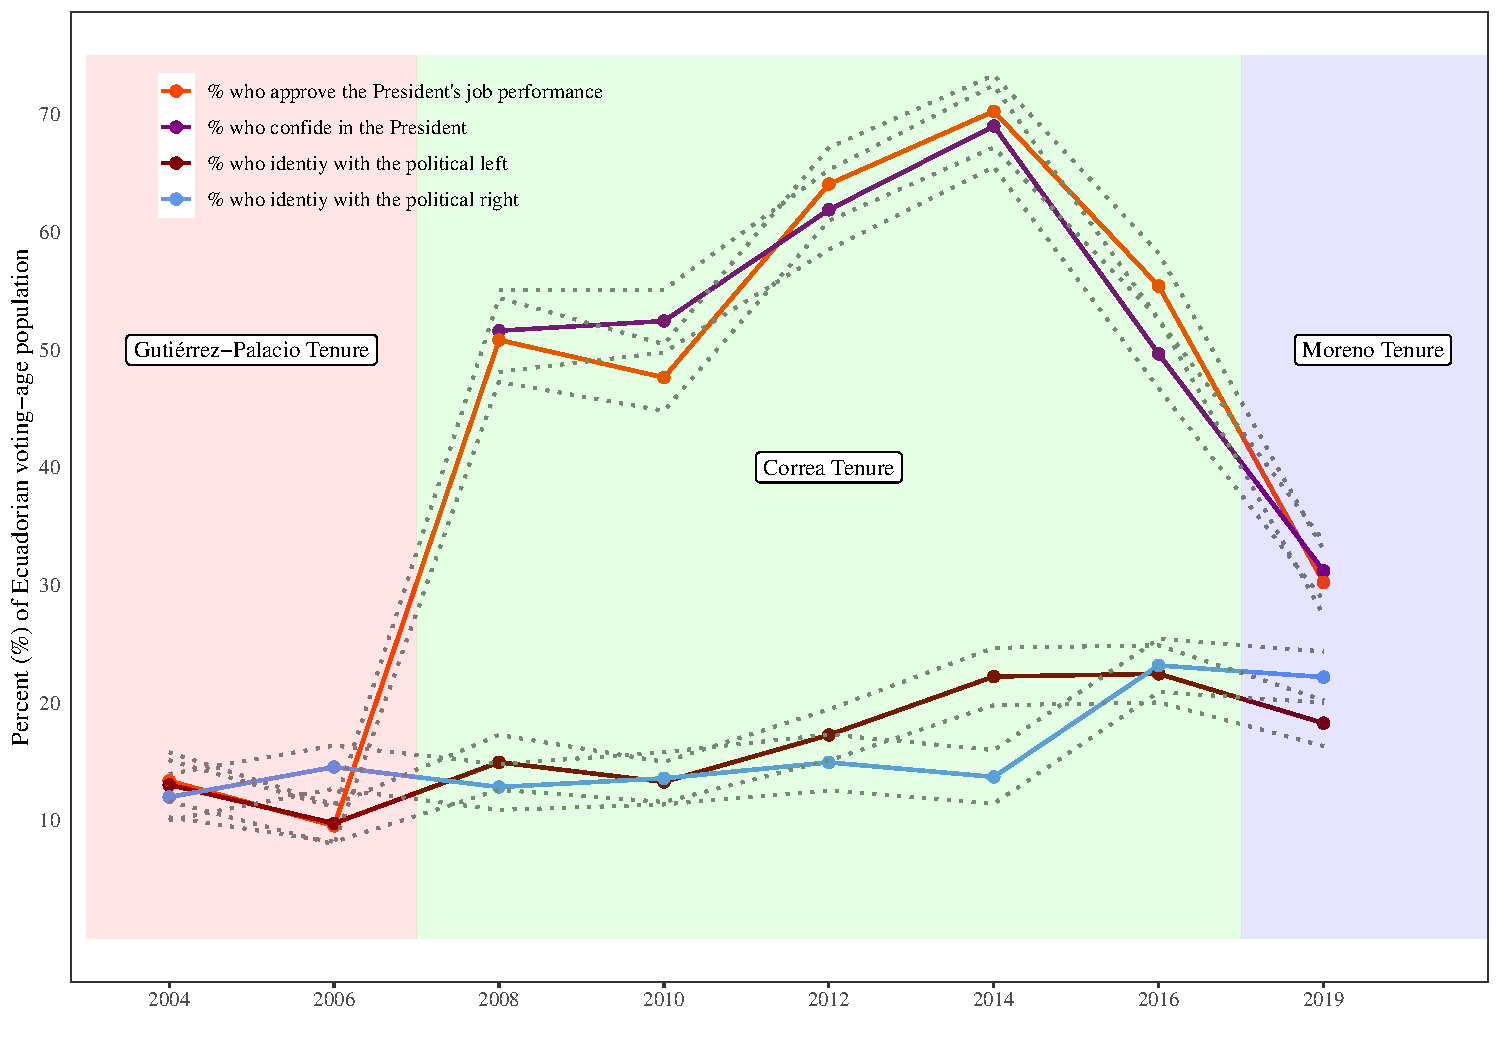
\includegraphics[width=\maxwidth]{figure/political_graph-1} 

}


\end{knitrout}
\caption{Ecuadorian public opinion indicators, 2004-2019}
\label{fig:ecua_pol}
Time series for political public opinion questions asked in the AB. Error bars show 95\% design-adjusted confidence intervals.
\end{figure}

However, as Ecuador entered a severe recession due to plunges in commodities’ prices and a fatal earthquake, the Correa administration was forced to take austerity measures, which were widely unpopular. Figure \ref{fig:ecua_ec} displays economic conditions and perceptions. After a decade of significant reform through public investment, progress seemed to have stopped as decreased public revenues did not allow for the considerable amount of government programs which had helped construct Correa's popularity. A significant amount of corruption accusations appeared against top government officials, which planted the seed of a deep investigation about a complex corruption scheme involving top government officials and large corporations \parencite{Villavicencio.2019}, which ended in a capture order for Correa in 2020. Several narratives started to be constructed by government officials to explain the flaws and weaknesses that had been denounced at that point. These included reducing corruption accusations to \enquote{political persecution} or unfounded claims done because of upcoming elections \parencite{Melendez.2017}. 

Regarding the economic recession, \textcite{Orozco.2015} holds that although the commodity price collapse in 2008 was greater, there was little reduction in economic activity as the country had greater possibilities of international financing and savings left over from past oil funds, which were used to keep government expenditure high. In 2016, as savings eroded and government debt had grown bigger, the economy stagnated significantly for the first time in the Correa administration. A weakened Correa left Ecuador for Belgium in 2017, after giving up power to his political successor, Lenín Moreno, who later turned his back on Correa.

Any kind of analysis about that the corruption tolerance increase during the 2014-2016 period must necessarily account for the events that happened at the time, most clearly indicated by figures \ref{fig:ecua_pol} and \ref{fig:ecua_ec}. In the next section, I analyze the related literature to construct a framework that will allow me to use these events as potential determinants for corruption tolerance at the individual level. 

% Here I create my graph, but I need to load some libraries first and create the data needed for my graphs.

% Now I do the graph:
\begin{figure}[htbp!]
\begin{knitrout}
\definecolor{shadecolor}{rgb}{0.969, 0.969, 0.969}\color{fgcolor}

{\centering 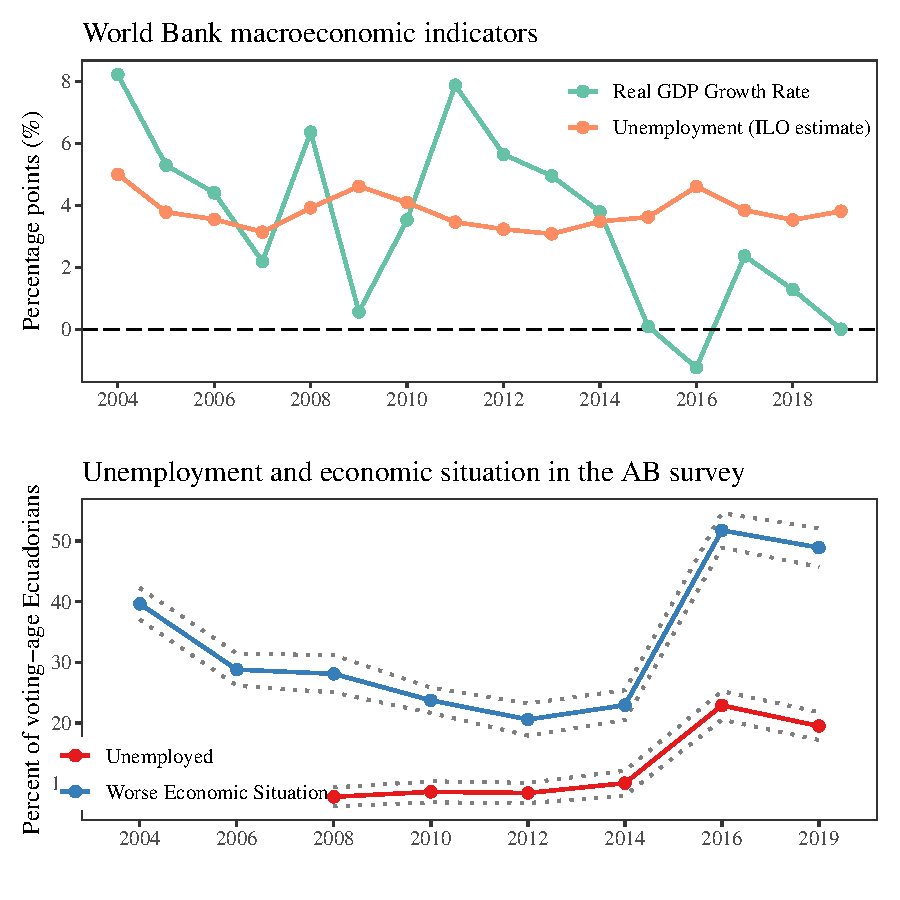
\includegraphics[width=\maxwidth]{figure/econ_graph-1} 

}


\end{knitrout}
\caption{Ecuadorian economic conditions 2004-2019}
\label{fig:ecua_ec}
Time series line graphs showing key economic indicators for the country (2004-2019). Real GDP growth and unemployment rates extracted from the World Bank's World Development Indicators. WTI oil barrel prices extracted from FRED.
\end{figure}
\end{document}
